%\newcommand{\ans}[1]{}
\documentclass[11pt]{article}
\usepackage{fullpage,pst-all,epsfig}

\usepackage{algorithmic}
\usepackage{algorithm}

\usepackage[margin=1in]{geometry}% http://ctan.org/pkg/geometry
\usepackage{lipsum}% http://ctan.org/pkg/lipsum
\usepackage{graphicx}

\usepackage{caption}
\usepackage{subcaption}

\newcommand{\comment}[1]{}
\newcommand{\Le}{\textbf{L}}

%\newcommand{\ans}[1]{\emph{Solution: #1}}
\newcommand{\ans}[1]{}

\newcommand{\seq}[1]{ \langle #1,\cdots \, \rangle}
\newcommand{\seqi}[1]{ \langle #1 \rangle}
	
\begin{document}
\thispagestyle{empty}
\begin{center}
\def\handout{Final Examination}
\vspace*{-.75in}
{\large University of New Mexico}\\
{\large Department of Computer Science}\\
\vspace*{0.5in}
{\LARGE {\bf \handout}}\\
\vspace*{0.1in}
{\large CS 561 Data Structures and Algorithms}\\
{\large Fall, 2012}\\ [0.3in]
\end{center}
 
\vfill

\makeatletter
\long\def\hint#1{({\em Hint\/}: #1)}
% \def\@oddhead{\rm\makebox[0in][l]{CS 461 Midterm ---Fall,
% 2003}\hfil\thepage\hfil\makebox[0in][r]{Name:\rule[-0.1in]{2in}{.5pt}}}
\let\@evenhead\@oddhead
\def\@oddfoot{}
\let\@evenfoot\@oddfoot

\def\problem#1{\def\problemheading{#1}\clearpage\item{\bf #1}}

% Comment out the above 'problem' def and use the one below to get
% all the problems on a single page, instead of page break each time.
%\def\problem#1{\def\problemheading{#1}\item{\bf #1}}

\def\extrapage{\addtocounter{enumi}{-1}\clearpage\item{\bf \problemheading, continued.}}

\let\part\item
\renewcommand{\theenumii}{\alph{enumii}}
\makeatother
\parindent 0pt

\vfill
\centerline{
\Large
\begin{tabular}{|l|}  \hline
Name: \hspace*{2in} \\ \hline
Email: \hspace*{2in}\\ \hline
\end{tabular}
}
\vfill

\hrule
\begin{itemize}

\item This exam lasts 2 hours.  It is open book and open notes but no electronic devices are permitted.

\item {\em Show your work!}  You will not get full credit if we cannot figure out how you arrived at your answer.  

\item Write your solution in the space provided for the corresponding problem.

\item If any question is unclear, ask for clarification.

\end{itemize}
\hrule
\vfill
\centerline{
\Large
\begin{tabular}{|c|c|c|c|}  \hline
Question & Points & Score & Grader \\  \hline\hline
1 & 20 & & \\  \hline
2 & 20 & & \\  \hline
3 & 20 & & \\  \hline
4 & 20 & & \\  \hline
5 & 20 & & \\  \hline
\hline Total & 100 & & \\  \hline
\end{tabular}
}
\vfill

\newpage

\begin{enumerate}
 

\problem{Short Answer}
 
Answer the following questions using \emph{simplest possible} $\theta$ notation.  Draw a box around your final answer.  No need to justify answers for problems on this page.
 
 \begin{enumerate}

\item If a data structure supports an operation ``foo'', such that $n$ calls to ``foo'' take $\theta(n \log n)$ time, what is the amortized cost of ``foo''?  \ans{It is $\theta(\log n)$} \\ \ \\ \ \\ \ \\ \ \\

\item How many bits are needed to write the number $n!$ in binary? \ans{$\theta(n \log n)$}  \\ \ \\ \ \\ \ \\ \ \\


\item $\sum_{i=1}^{n} \frac{i}{n}$ \ans{$\theta(n)$}  \\ \ \\ \ \\ \ \\ \ \\

\item Fastest time to find the \emph{longest} path in a directed graph, $G$, with no cycles, and where all edge weights are positive.  Assume there are $n$ nodes in $G$ and $m$ edges and give your answer in terms of $n$ and $m$. \ans{$\theta(nm)$} \\ \ \\ \ \\ \ \\ \ \\

\item Suppose you have a hash function that hashes $n$ items into an array of length $m$.  What is the expected number of colliding pairs of elements (asymptotically, as a function of $n$ and $m$)?
\ans{$\theta(n^{2}/m)$}

\pagebreak

\item Assume you have a graph with $n$ nodes and $m$ edge.  Assume further that you have a set-union data structure which somehow ensures all operations are $O(1)$ amortized time.  What is the new runtime of Kruskal's algorithm? \ans{It is still $\theta(m \log n)$.} \\ \ \\ \ \\ \ \\ \ \\

\item Assume you have a graph with $n$ nodes and $m$ edge.  Assume further that you have a heap data structure which somehow ensures all operations are $O(1)$ amortized time.  What is the new runtime of Prim's algorithm?  \ans{It is now $\theta(m+n)$.} \\ \ \\ \ \\ \ \\ \ \\

\item Assume you have a graph with $n$ nodes and $m$ edge.  What is the fastest time to determine if the graph has a cycle of odd length?  \ans{It is $\theta(n+m)$} \\ \ \\ \ \\ \ \\ \ \\

\item Imagine you have two skip lists, each containing $n$ distinct items.  What is the expected time to merge them into a new skip list over all $2n$ of the distinct items?  The new skip list should be able to support all skip-list operations with the same time costs as for any skip lists over $2n$ items. 

\ans{$\theta(n)$.  Need to merge lists $L_{1}$ to $L_{x}$ where list $L_{i}$ contains $n/2^{i}$ records in expectation.  The cost of the merge is thus $n/2^{i-1}$.  Summing from $i = 1$ to $\infty$, we get cost $\theta(n)$} \ \\ \ \\ \ \\ \ \\ \ \\

\item Solution to the following recurrence relation: $f(n) = 2f(n-1) - f(n-2) + 1$. \ans{$\theta(n^{2})$ or $\theta(c_{1}n^{2} + c_{2}n + c_{3})$.  Annihilator is $(L - 1)^{3}$.} \\ \ \\ \ \\ \ \\ \ \\


\end{enumerate}


\problem{Short Answer}

\begin{enumerate}

\item Prof. Goofus conjectures that if there is a graph $G$ such that 1) $G$ contains all possible edges (i.e. it is a clique) and 2) each edge in $G$ has a unique weight, then the minimum spanning tree for $G$ will always contain the $n-1$ lightest edges of $G$ (where $n$ is the number of nodes in $G$).  Show Goofus is wrong by drawing a weighted graph and  giving a MST for that graph that disproves the conjecture. \ans{Nodes are a,b,c, d and e.  Edges are (a,b), (b,c) (a,b), (d,e) with weight 1, (b,d) with weight 10.  The MST always contains the edge (b,d).} \\ \ \\ \ \\ \ \\ \ \\


\pagebreak

\item Consider the following problem about sending a message in a wireless network that is under attack.   Assume there are $n$ times steps, and Alice sends in $c\sqrt{n}$ of these steps selected uniformly at random, and Bob listens in $c\sqrt{n}$ of these steps selected uniformly at random.  Further there is an adversary that jams $n/2$ of the time steps selected uniformly at random.  A step is said to be \emph{good} if 1) the step is not jammed; 2) Alice sends in the step; and 3) Bob listens in the step.  What is the expected number of good time steps?  How large should $c$ be to ensure that the expected number of good steps is least one?

Hint: Linearity of Expectation.

\ans{For each step $i$, let $X_{i}$ be an r.v. that is $1$ if the step is good and $0$ otherwise.  Note that $E(X_{i}) = (c/\sqrt{n})(c/\sqrt{n})(1/2)  = c^{2}/2n$.  Let $X$ be the total number of good steps.  By linearity, $E(x) = n (c^{2}/2n) = c^{2}/2$.  Thus we want $c \geq \sqrt{2}$ to ensure that the expected number of good steps is at least $1$.}


\end{enumerate}





\problem{Graph Coloring} A $3$-regular undirected graph is a graph, $G=(V,E)$ where every node has exactly $3$ neighbors.  Recall that to properly color a graph, you must assign a color to each vertex of the graph so that every edge in $E$ connects vertices with two different colors.

Prove by induction that any $3$-regular graph can be colored with $4$ colors.  Prove this by induction on $n$, the number of vertices in $G$. Don't forget to include the Base Case (BC), Inductive Hypothesis (IH) and Inductive Step (IS).  Hint: Remember in the IS to create a {\bf smaller} subproblem and to use the IH to solve it.  

\ans{We show something a bit stronger: For any graph $G$ where each node has degree at most $3$, $G$ is 4-colorable.  BC: If $n$ = 1 then clearly the graph can be colored with $4$ colors.  IH: For any $j<n$, a $3$ regular graph with $j$ nodes can be colored with $3$ colors.  IS: Let $v$ be some vertex in $G$.  Let $G'$ be the graph you get by removing $v$ and all its edges from $G$.  Note that $G'$ is 3-regular and has $n-1$ vertices.  Thus, by the IH, $G'$ can be colored with at most $4$ colors.  Now if we add $v$ back in, we see that it has exactly $3$ neighbors, which can be colored with at most $3$ different colors.  Hence, there is an extra color available that we can color $v$ with in order to get a $4$ coloring of $G$.}


\problem{Debs and Poodles}

There are $n$ debutants (debs) and $m$ poodles.  Each deb $i$ has a quota $n_{i}$ of poodles that she can adopt.  Each poodle $j$ has a set $S_{j}$ of debs it prefers.  Your goal is to assign poodles to debs in such a way that no deb exceeds her quota of poodles, and each poodle $j$ is matched with exactly one deb in its set $S_{j}$.

\begin{enumerate}

\item Show how you can use Max-flow to find an assignment if possible.  What is the worst case runtime of your algorithm (you can use $F(v,e)$ to denote the runtime of max flow on a graph with $v$ nodes and $e$ edges).
\ans{Create a graph $G$ containing a vertex for each deb, a vertex for each poodle and a source vertex $s$ and sink vertex $t$.  Add edge from $s$ to each deb vertex $i$ with capacity $n_{i}$.  Add edge from each deb $i$ to poodle $j$ with capacity $1$ if $i \in S_{j}$.  Finally add edge from each poodle $j$ to $t$ with capacity $1$.  Now find the max-flow in this graph.  This takes time $F(n+m,nm)$}

\pagebreak


\item You run the algorithm from part a) and unfortunately do not find a assignment that meets the criteria.  The debs believe your algorithm is correct but they believe your implementation of it has a bug.  Based on your understanding of max-flow, how can you prove to the debs that your program is correct and that no assignment is possible?  Your proof strategy must work for every instance where there is no assignment.

\ans{If there is no flow of size $m$, then there is a cut of capacity less than $m$ in the graph.  This gives a set $P$ of poodles such that the quota of the set of debs, $D(P)$ they are willing to be adopted by is smaller than the set $P$.  Thus, the set $P$ and $D(P)$ is a proof that no assignment is possible.}

\end{enumerate}



\problem{Sensor Networks}

Your boss presents you with the following problem.  You are given a graph $G = (V,E)$ that represents a sensor network.  The nodes of $V$ represent sensors, and each node $v \in V$ has a positive weight $w(v)$ that indicates the importance of the data collected by that sensor.  There is an edge $(u,v) \in E$ if sensors $u$ and $v$ are neighbors in the network, and in such a case, $u$ and $v$ can not both be turned on because of interference issues.  You want to turn on a subset of the nodes with maximum total weight that avoids any interferences.

Your goal is thus to find a subset $S \subseteq V$ such 1) no two nodes in $S$ are neighbors; and 2) the sum of the weights of all nodes in $S$ is maximized among all such sets.

Your boss thinks this problem is pretty easy, but decides to be generous and give you the entire weekend to work on it.

\begin{enumerate}

\item Show that this problem is NP-Hard by a reduction from one of the following NP-Hard problems: 3-SAT, CLIQUE,  INDEPENDENT SET, VERTEX COVER, 3-COLORABLE or HAMILTONIAN CYCLE.
\ans{This is NP-Hard by a reduction from INDEPENDENT-SET.  Let $G=(V,E)$, $k$ be an INDEPENDENT-SET problem.  Imagine we have an algorithm, A, that can solve the above problem.  Then assign weight $1$ to each node in $V$ and feed this problem to algorithm $A$.  $G$ has an independent set of size $k$ iff $A$ returns a set $S$ with total weight at least $k$.} \ \\ \ \\ \ \\ \ \\ \ \\ \ \\ \ \\ \ \\ \ \\ \ \\ \ \\

\pagebreak

\item Now your boss decides to create a new easier problem by assuming that $G$ is a path (see Figure~\ref{f:path}).  He claims that the following greedy algorithm will find an optimal set $S$ for this new problem.  GREEDY initially starts with an empty set $S$.  Then it repeats the following until the set $V$ is empty: 1) find a vertex $v \in V$ of maximum weight; 2) add $v$ to $S$; and 3) remove all neighbors of $v$ from $V$.

Show your boss is wrong by giving a problem instance (a graph $G$ that is a path, and weights for the vertices of $G$), such that GREEDY does not return the optimal solution for that problem.

\begin{figure}[h]
\begin{center}
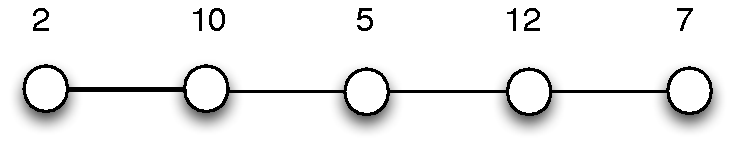
\includegraphics[scale=0.4]{path.pdf} 
\caption{}
\label{f:path}
\end{center}
\end{figure}

\ans{Consider the graph $V = \{a,b,c\}$ where $E = \{ (a,b), (b,c) \}$ $w(a) = w(c) = 2$, $w(b) = 3$.  Greedy will always take the node $b$, but the optimal solution takes the nodes $a$ and $b$.} \ \\ \ \\ \ \\ \ \\ \ \\ \ \\ \ \\ \ \\ \ \\ \ \\ \ \\ \ \\


\pagebreak

\item Now describe how to solve this new problem (where $G$ is a path) using dynamic programming.  Let the vertices in the path have labels $v_{1}$, \ldots, $v_{n}$.   Let $m(i)$ be the max weight of the set $S$ that is obtainable by considering only vertices $v_{1}$ through $v_{i}$.  First give the recurrence relation (and base case(s)) for $m(i)$ below.

\ans{$m(0) = 0$, $m(1) = w(v_{1})$.  For all $i>0$, $m(i) = \max (m(i-1), m(i-2) + w(v_{i}))$. } \ \\ \ \\ \ \\ \ \\ \ \\ \ \\ \ \\ \ \\


\item Now describe how to create a dynamic program to find $S$.  What is the run time of your algorithm as a function of $n$?

\ans{It is necessary to have an array $m$ that is filled in from left to right using this recurrence above.  We can also create backward edges from $i$ to either $i-1$ or $i-2$ depending on whether or not the maximum value for $m(i)$ was achieved using $m(i-1)$ or $m(i-2)$.  Then to reconstruct the set $S$, we simply start at the value $m(n)$ and follow the edges backwards to $m(0)$.  Every time we visit a vertex $v_{i}$ in this path, we output it as being part of $S$.  The runtime of this algorithm is $O(n)$. }

\end{enumerate}


%\extrapage



 
 
 
 


\end{enumerate}

  
  
 
  \end{document}
 
 
   \problem{Recurrences and Asymptotics}
 
 Remember that when the base case for a recurrence is not explicitly given, assume that it is constant for inputs of constant size.
 
 \begin{itemize}
 
 \item Consider the recurrence $f(0) = 1$, $f(n) = \sum_{i=0}^{n-1} f(i)$.  Prove that the solution to this recurrence is $\theta(2^{n}$)
 
 \ans{This is a straightforward proof by induction.}
 \ \\ \ \\  \ \\ \ \\ \ \\  \ \\ \ \\ \ \\  \ \\ \ \\ \ \\  \ \\ \ \\ \ \\  \ \\ \ \\ \ \\  \ \\

\item Solve the following recurrence: $f(n) = 4f(n-1) - 4f(n-2) + 2^{n}$.  Do not solve for the constant coefficients
\ans{$(L^{2}-4L+4) = (L-2)^{2}$ annihilates the homogeneous part and $(L-2)$ annihilates the non-homogeneous part.  So the annihilator is $(L-2)^{3}$ and hence the solution is $(c_{1}n^{2} + c_{2} n + c_{3}) 2^{n}$}
 \ \\ \ \\  \ \\ \ \\ \ \\  \ \\ \ \\ \ \\  \ \\ \ \\ \ \\  \ \\

\pagebreak


\item Solve the following recurrence: $f(n) = f(n/2) + f(n/4)$.  Do not solve for the constant coefficients.  If an algorithms runtime is given by this recurrence, how would it compare with algorithms with runtimes of $\theta(2^{n})$, $\theta(n)$, $\theta(\sqrt{n})$?

 \ans{Let $2^{i}=n$ and $F(i) = f(2^{i})$.  Then we get a transformed recurrence: $F(i) = F(i-1) + F(i-2)$, whose solution is  $F(i) = c_{1} \phi^{i} + c_{2} \hat{\phi}^{i}$. Reverse transforming this solution, and using the fact that $i = \lg n$ we get  
 $f(n) = n^{\lg \phi} + n^{\lg \hat{\phi}}$.  This solution is approximately $\theta(n^{.694})$, so it is better than linear but worse than square root run time.}
 \ \\ \ \\  \ \\ \ \\ \ \\  \ \\ \ \\ \ \\  \ \\ \ \\ \ \\  \ \\
 
 \end{itemize}

\problem{Heaps and Sorting}

Professor Humbert claims to have invented a new Max-Heapify function for heaps that runs in $O(\lg \lg n)$ time.  Moreover, Humbert claims that his new Max-Heapify function is completely comparison based, i.e. the only way it ever compares two keys is with the $\leq$ operator.  Could Humbert be right?

\ans{No.  If such a Max-Heapify function existed, we could plug it into heap sort and use if to do comparison-based sorting in $\Theta(n\lg \lg n)$ time. }

 \ \\ \ \\ \ \\  \ \\ \ \\ \ \\  \ \\ \ \\ \ \\  \ \\

Prove that the following algorithm correctly sorts a list of $n$ elements by induction on $n$.  Don't forget to include the base case, inductive hypothesis and inductive step.
\begin{verbatim}
SillySort(A, i, j){
  Let n = j - i + 1;                   // n is the number of elements to sort
  If n <= 1 then return;          //nothing to sort
  If n == 2                              // only two elements to sort
    then
      if A[i] > A[j], swap A[i] and A[j]
  else                                     // more than two elements to sort                    
     SillySort(A,i+n/2,j);         //SillySort the last n/2 elements of A
     SillySort(A,i,i+n/2);    //SillySort the first n/2+1 elements of A
     SillySort(A,i+1,j)             //SillySort the last n-1 elements of A
 }
\end{verbatim}

\extrapage

\ans{Prove by induction on the size of L.  Need to first prove that the minimum element in the array winds up in the first position.}

\problem{Data Structures}

\begin{itemize}

\item Imagine that in a red black tree, the rule that a red node must have two black children is relaxed to the rule that a red node must have at least one black child.  All other rules remain the same.  What is now the maximum asymptotic height that a red black tree with $n$ nodes can have?  Give an example or proof as necessary to justify your claim.

\ans{The tree can now have $\theta(n)$ height.  Imagine one branch where all the nodes are red except for the root, and one child of each node on the branch - the final node in this branch has two black children.}

\pagebreak

\item Imagine you have a ``blacklist'' of $n$ messages that are spam.  When a new message arrives in your mail queue, you want to test it to see if it's a message in your black list.  However, space is at a premium and so you don't want to have to store all $n$ messages in memory (assume each message is many bits in length).  Answer the following questions with asymptotic notation.  Hint: Assume that you have a hash function that maps strings of any size to integers that are essentially random.
\begin{itemize}
\item What is the minimum number of bits of space to ensure that you can test if new messages are in the blacklist and get false positive with probability no more than $1/100$?  What is the time needed to test if a message is in the blacklist in this case?
\item How many bits do you need if you want the probability of false positives to be no more than $1/n$?  What is the time to test membership in this case?
\end{itemize}
\ans{Use a Bloom filter.  You need $\theta(n)$ bits and $\theta(1)$ time in the first case (since $k = \theta(1)$).  In the second case, you need 
$\theta(n \lg n)$ bits (since $m$ must be $n \lg n$) to get probability of false positives less than $1/n$; you need $O(\lg n)$ time since $k$ is $O(\lg n)$}

\end{itemize}

 \problem{Probability}
 
 \begin{itemize}
 \item \emph{Bad Santa II: Mr. Kringle's Revenge:} Consider the Bad Santa problem from hw1 with the following change.  The child is allowed to take $2$ passes over the sequence of boxes if necessary, but still needs to find just one present before stopping.  However, Santa can secretly hide the presents again after the first pass of the child.  Describe and analyze an algorithm for this new problem that minimizes the expected number of boxes opened.  Hint: The problem is now much easier than the hw problem.
 
 \ans{The algorithm: In this first pass, choose $\log n$ boxes uniformly at random and open those.  In the second pass, just open all boxes from let to right until finding a present.  The expected number of boxes opened is no more than $\log n + (1/n)n$, since the probability of getting to the second pass is only $(1/2)^{\log n} = 1/n$.  Thus the expected number of boxes opened is $O(\log n)$.}
 
 \pagebreak
 
 \item \emph{Closest Points:} Imagine $n$ points are distributed uniformly at random on a circle with circumference $1$.  Show that the expected number of pairs of points that are within distance $\theta(1/n^{2)}$ of each other is greater than $1$ (note that this implies that the smallest distance between two points is likely $O(1/n^{2})$).  Hint: Partition the circle into $n^{2}/k$ regions of size $k/n^{2}$ for some constant $k$; then use the Birthday paradox to solve for the necessary $k$.
 \ans{Think of the regions as bins and the points as balls.  The probability that two points fall in the same region is $k/n^{2}$.   Let $X_{i,j}$ equal $1$ if points $i$ and $j$ fall in the same region and $0$ otherwise and let $X$ be the sum over all $n \choose 2$ values $i$ and $j$ of $X_{i,j}$.  Using linearity of expectation, $E(X) = {n \choose 2}k/n^{2}$.  Thus, for some $k$, e.g. $k\geq 3$, we would expect at least one pair of balls to fall in the same bin.}

\end{itemize}


 \problem{Are you Smarter than a 561 Student?}
 
You are competing in the popular game show ``Let's Make a Dynamic Program'' with another player.  You and your opponent both start with $0$ dollars.  If you reach (or exceed) $n$ dollars before your opponent, you win $n$ dollars; if your opponent reaches (or exceeds) $n$ dollars before you, you win nothing; and if you both reach (or exceed) $n$ dollars at the same time, you both win $n$ dollars.  In each turn, you get to choose the level of difficulty of the next question asked, where this difficulty is represented by an integer $k$ between $1$ and $n$.  If you answer the question correctly, you get $k$ dollars, otherwise your opponent gets $k$ dollars.  Note that you are always in control throughout the entire game of the difficulty level of the question asked.
 
Through careful study of the game you have been able to determine the probability $p_{i}$ for $i$ between $1$ and $n$, which is the probability that you will answer a question of difficulty $i$ correctly.

\begin{itemize}

\item Consider the greedy algorithm where you always choose a question of difficulty level $i$ for $i$ maximizing $i*p_{i} - i*(1-p_{i}) = i(2p_{i}-1) $.  Is this an optimal algorithm?  Hint: Is it ever better to make a long shot bet because the probability of success from multiple short bets is small.  In particular,think about the case where your opponent has $n-1$ dollars and you have $0$.


\ans{Greedy is not optimal.  Consider the case where $p_{1} = 1/4$, $p_{n} = 1/5$ and for all other $i$, $p_{i} = 0$.  Then $1$ is the difficulty level maximizing the expected difference between you and your opponent, since $1p_{1} - 1q_{1} = -1/2$ and $np_{n} - nq_{n} = -(3/5)n$.  Assume further that your opponent has $n-1$ dollars and you have $0$ dollars.   If you choose a difficulty of $n$, you have the chance of jumping ahead of your opponent to victory, which happens with probability at least $1/5$.  In contrast, the probability of success by following the greedy strategy, where you just keep choosing difficulty of $1$ will only be $(1/4)^{n}$, which is exponentially small in $n$.}

\pagebreak

\item Let state $(i,j)$ be the state where you have $i$ dollars and your opponent has $j$ dollars.  Note that if you choose the difficulty level to be $k$ at that state, you have probability $p_{k}$ of going to state $(i+k,j)$ and probability $(1-p_{k})$ of going to state $(i,k+jj)$.  Now let $e(i,j)$ be your expected winnings if you have $i$ dollars and your opponent has $j$ dollars and you play optimally.  Write a recurrence relation for the value $e(i,j)$.  Note: You will find it useful to consider $i$ and $j$ values that range from $0$ to $2n-1$.  Hint: Use expected values for simpler subproblems and the probabilities $p_{i}$ described above to compute $e(i,j)$.  Don't forget the base case(s).

\ans{Base Cases: $e(i,j) = n$ for all $j \geq n$.  $e(i,j) = 0$ for all $i \geq n$ and $j < n$.  \\ Recurrence:  for other values of $i$ and $j$,
 $e(i,j) = max_{1 \leq k \leq n} p_{k} e(i+k,j) + (1-p_{k}) e(i,j+k)$}

\pagebreak


\item Give the pseudocode for computing the value $e(0,0)$, which gives you your expected winnings if you play this game optimally.
\ans{Basically, need to fill in the base case first of a n by n array and then fill in the remaining values from bottom up and right to left}
  
\pagebreak 

\item What if the game is changed as follows.  You still select the difficulty level $k$, but after your selection, both you and your opponent have the chance to write down the answer to the question.  Whoever gets the answer correct wins $k$ dollars (note that both of you may win now).  There is no penalty for a wrong answer.  The probability that you answer a question of difficulty $k$ correctly is $p_{k}$ and the probability that your opponent answers correctly is $q_{k}$.   Can you still solve this new problem using dynamic programming?  If so, give a recurrence and describe how to change the algorithm.  If not, describe why not.

\ans{It is still possible.  The base case for the recurrence is the same as before.  The new part of the recurrence is determined by following equation for fixed $k$:
$e(i,j) =  (p_{k}q_{k} e(i+k,j+k) + (1-p_{k})q_{k}e(i,j+k) + p_{k}(1-q_{k})e(i+k,j) + (1-p_{k})(1-q_{k}) e(i,j)$.  Note that $e(i,j)$ appears on both the left and right side of this equation, which at first seems to cause problems in formulating a recurrence; however, it is still possible to isolate $e(i,j)$ on the left side.  Then it is possible to get a proper recurrence by taking the maximum over all possible values of $k$.  The recurrence and pseudocode is left as an exercise.}
  
 \end{itemize}
  
  \end{enumerate}
  

 
 
 \problem{Borges Library - determining if all the books in a given room are the same}
1) Create a Bloom Filter for all the books in the room
 
2) How to compare two rooms quickly to determine if they have the same set of books or not.


 
 
\problem{Data Structure Problem (BST, skip list, etc, heap)}
 
 
 
 \problem{Bday}
  
 \problem{Hafts}
 
 
 \problem{Skip Lists}
 
 \begin{itemize}
 \item How would you merge two skip lists?
 \item How would you find the $i$-th element in sorted order
 
\end{itemize}

 
 
\problem{Search Trees}

Consider a tree with the following properties:

\begin{itemize}
\item Each internal node has exactly three children
\item The heights of the subtrees rooted at each child differ by at most $1$.
\end{itemize}

What is the maximum height of such a tree containing $n$ nodes?

Hint: Write a recurrence relation for the maximum number of nodes as a function of the height and then solve for the height.  Show your work!

\ans{Let $T(h)$ be the maximum number of nodes in a tree of height $h$.  Then $T(h) = T(h-1) + 2 T(h-2) + 1$.  $(\Le^{2}-\Le - 2) = (\Le -2)(\Le +1)$ annihilates the homogeneous part and $\Le - 1$ annihilates the non-homogeneous part.  Thus, the solution is of the form $T(h) = c_{1}2^{h} + c_{2} + c_{3} (-1)^{h}$.  Let $n$ be the number of nodes in the tree.  We know that $n \geq T(h)$ and so $n \geq c_{1}2^{h} + c_{2} + c_{3} (-1)^{h}$.  If we let $c = c_{2} - c_{3}$, we can say that, $n \geq c_{1} 2^{h} + c$.  Taking logs of both sides, we have that $\log n \geq h \log (2c_{1}) + \log c$.  This implies that $h \leq 1/(log(2c_{1}))(\log n - \log c)$.  The right hand side is $O(\log n)$.  Thus, $h$ is $O(\log n)$.}

\problem{Hash Tables and Probability}

Assume we hash $n$ items into a hash table with $n$ bins using a good hash function i.e. each item is hashed to a bin chosen independently and uniformly at random.  Give a good upper bound on the number of empty bins.  Solve for the constants in your upper bound i.e. do not use asymptotic notation.

Hint: Use the fact that $1-x \leq e^{-x}$ for all $x$.

\ans{Let $X_{i}$ be an indicator random variable which is $1$ if the $i$-th bin is empty and is $0$ otherwise.   Then note that $E(X_{i})$ equals the probability that the $i$-th bin is empty.  This is the probability that the $n$ items do not fall in bin $i$.  The probability that a single item does not fall in bin $i$ is exactly $1 - 1/n$.  Since the items are all hashed independently, the probability that \emph{no} item hashes into bin $i$ is exactly $(1-1/n)^{n}$.  Using the hint, note that  $(1-1/n)^{n} \leq (e^{-1/n})^{n} = e^{-1}.$  Let $X$ be a random variable giving the number of empty bins and note that $X = \sum_{i=1}^{n} X_{i}$.  Using linearity of expectation, we see that $E(X) = E(\sum_{i=1}^{n} X_{i}) = \sum_{i=1}^{n} E(X_{i}) \leq n/e$.  Thus the expected expected number of empty bins is at most $n/e$.  This is actually a pretty tight upper bound as $n$ gets large.}

\problem{Divide and Conquer}

Imagine that after graduating from UNM, you start your new job at the exciting investment banking firm SELLOUT, Inc.  The firm if faced with the following problem: they have an array of the predicted prices of a stock over $n$ days and they want to determine, using this array, exactly one day to buy the stock and one day to sell the stock in order to maximize their profit.

The problem can be formally stated as follows.  You are given an array $A$ of $n$ numbers.  You want to choose indices $1 \leq i < j \leq n$ such that $A[j] - A[i]$ is maximized over all such indices.  Give an $o(n^{2})$ algorithm to solve this problem.

\ans{Use Recursion!  Recursively find the pair of indices $i_{l}$ and $j_{l}$ on the left half of the array such that $i_{l} < j_{j}$ and $A[j]-A[i]$ is maximized over all such pairs.  Find a similar pair $i_{r}$ and $j_{r}$ on the right half of the array.  Now find $x$, the index of the element with smallest value on the left half and $y$, the index of the largest element on the right half.  Finally, return 
max($A[j_{l}] - A[i_{l}]$, $A[j_{r}] - A[i_{r}]$, $A[y] - A[x]$).  The run time of this algorithm is given by the same recurrence as for merge sort $T(n) = 2T(n/2) + n$, whose solution is $n \log n$.  Note that we can get an even faster algorithm than this using dynamic programming. Also there is another $O(n \log n)$ solution that makes use of a heap or BST.}

\end{enumerate}

\end{document}





% \item {\bf True or False}:  In a max-heap, the element with smallest key is always at the
% rightmost leaf node of the heap? \ans{F: it's always at a leaf node
% but not necessarily the rightmost leaf node}
% \item {\bf True or False}:  Bubblesort requires $O (n)$ extra space (not counting the space
% to store the array to be sorted)? \ans{F: it takes $O (1)$ extra space}
% \item {\bf True or False}:  $1/\log n$ is $o (1)$? \ans{T}
% \item {\bf True or False}:  $\log \sqrt{n}$ is $\Theta (\log n)$?
% \ans{T: since $\log \sqrt{n} = 1/2\log n$}
% \item {\bf True or False}:  $2^{n-1}$ is $o (2^{n})$?\ans{F: since $2^{n-1}=1/2*2^{n}$}
% \problem{Annihilators}\\

% Consider the recurrence $T (n) = 2T (n-1) - T (n-2) + 4$, $T (0)=0$, $T (1)=0$.
% Solve this recurrence \emph{exactly} using annihilators.  Don't forget
% to check your answer.

% \ans{Consider the homogeneous part first.  Let $T_{n} = 2T (n-1) - T
% (n-2)$, and $T = \seqi{T_{n}}$.  Then
% \begin{eqnarray}
% T & = & \seqi{T_{n}}\\
% \Le T & = & \seqi{T_{n+1}}\\
% \Le^{2} T & = & \seqi{T_{n+2}}
% \end{eqnarray}
% Since $\seqi{T_{n+2}} = \seqi{2T_{n+1}-T_{n}}$, we know that
% $\Le^{2}T-2\Le T + T = \seqi{0}$, and thus $\Le^{2}-2\Le +1 = (\Le -1)
% (\Le -1)$ annihilates $T$.  Further we know that $(\Le -1)$
% annihilates the non-homogeneous part.  Thus the annihilator of the
% whole sequence is $(\Le -1)^{3}$.  Thus $T (n)$ is of the form:
% \[
% T (n) = c_{1}n^{2}+c_{2}n+c_{3}
% \]
% We know:
% \begin{eqnarray}
% T (0) = 0 & = & c_{3}\\
% T (1) = 0 & = & c_{1} + c_{2}\\
% T (2) = 4 & = & 4 c_{1} + 2c_{2}
% \end{eqnarray}
% so $c_{1}=2$, $c_{2}=-2$, $c_{3}=0$ and thus
% \[
% T (n) = 2n^{2}-2n
% \]
% Check: $T (3) = 2*4-0+4=12$ and $2*9-6=12$.}




% \problem{Substitution Method}\\
% Consider the following recurrence: $$T(n) = T(n-1) + T(n-2) - n + 3,$$
% where $T(1) = 1,T(2)=2$.\\ \ \\ Show that $T(n) = n$ by induction.
% Include the following in your proof: 1)the base case(s) 2)the
% inductive hypothesis and 3)the inductive step.

% \ans{Base Case: T(1) = 1.\\Inductive Hypothesis: For all $j<n$, T(j) =
% j\\Inductive Step: We must show that $T(n)=n$, assuming the inductive
% hypothesis.  
% \begin{eqnarray}
% T(n) & = & T(n-1) + T(n-2) - n + 3\\
% T(n) & = & (n-1) + (n-2) - n + 3\\
% T(n) & = & n
% \end{eqnarray}
% where the inductive hypothesis allows us to make the replacements in
% the second step.}

% \item {\bf True or False}: If $X$ and $Y$ are sequences that both
% begin with the character $a$, then some longest common subsequence of
% $X$ and $Y$ begins with the character $a$. \ans{True}
 \pagebreak

\item (5 points) Your boss wants to create the following data structure in the comparison model and to name it after himself, the \emph{Merkle}.  A Merkle has the following operations and properties on it.  BuildMerkle takes an arbitrary array and builds a Merkle from it in $O(n)$ time.  The resulting Merkle will provide the following operations.  FindMin (resp. FindMax) will return the minimum (resp. maximum) element and run in $O(\log n)$ time.  Successor(x) (resp. Predecessor(x)) return the next largest (resp. smallest) element in the Merkle after the element $x$, and both of these operations run in $O(1)$ time.  Intuitively, your boss wants you to combine the nice properties of the heap with the nice properties of a data structure like skip lists.  Can you immortalize your boss's name in CS textbooks by creating this data structure?

\ans{No.  This would allow sorting in $O(n)$ time.  To show this, first build the Merkle from an unsorted array, then find the minimum element and keep calling successor}



\pagebreak

In this problem, you will modify count-min sketches so that they handle negative counts.  As in class, assume you are presented with a stream of tuples of the form $(i_{t},c_{t})$, except now $c_{t}$ may be either a negative or positive integer.  The data structure you will use will consist of two count-min sketches, a positive count-min sketch for positive counts and a negative count-min sketch for negative counts.  In particular, each of the two sketches will use $m$ counters and $k$ hash functions, where all hash functions can be assumed to be independent.  If $c_{t}$ is positive, in the positive count-min sketch (positive sketch for short),  for each $1 \leq a \leq k$, $C_{a,h_{a}(i)}$ will be incremented by $c_{t}$.  If $c_{t}$ is negative, in the negative sketch, for each $1 \leq a \leq k$, $C_{a,h_{a}(i)}$ will be incremented by $-c_{t}$.   The estimate of the count of an item, $i$ at time $T$ is $m^{+}(i,T) - m^{-}(i,T$, where $m^{+}(i,T)$ is the value of the smallest counter associated with $i$ in the positive sketch and $m^{-}(i,T)$ is the value of the smallest counter associated with $i$ in the negative sketch.  As in class, let $Count(i,T)$ be the true count of item $i$ in the stream up to time $T$.  Also assume that $k = m \epsilon/e$ for the positive sketch and for the negative sketch.
 
 \item (7 points) Give a good bound on the probability that the following holds:\\
 $$ Count(i,T) - \epsilon \sum_{i=1}^{T} |c_{i}| \leq m(i,T) \leq Count(i,T) + \epsilon \sum_{i=1}^{T} |c_{i}| $$
 Please prove your bound.
 
 
 \ans{Let $S^{+}_{T}$ be the sum of all the positive counts in the stream up to time $T$.  For the positive sketch, we know that $Pr(Z_{j}> \epsilon S^{+}_{T}) \leq e^{m\epsilon/e}$, where $Z_{j}$ is the amount the min counter associated with $i$ in the positive sketch is incremented by items other than $i$.  Let $S^{-}_{T}$ be the sum of the absolute values of the negative counts in the stream up to time $T$.  Then we also know using the analysis in class that for the negative sketch, $Pr(Z'_{j}> \epsilon S^{-}_{T}) \leq e^{m\epsilon/e}$, where $Z'_{j}$ is the amount the min counter associated with $i$ in the negative sketch is incremented by items other than $i$.   A simple union bound on these two inequalities shows that $Pr(Z_{j}> \epsilon S^{+}_{T} \textrm{ or } Z'_{j}> \epsilon S^{-}_{T}) \leq 2 e^{m\epsilon/e}$.  Thus, we can see that $Pr(Z_{j} + Z'_{j} > \epsilon \sum_{i=1}^{T} |c_{i}|) \leq  2 e^{m\epsilon/e}$.  Thus the probability the approximation bound given holds is at least $1 - 2 e^{m\epsilon/e}$. }

\pagebreak

\item  (7 points) Now imagine you are given a constant number of data streams $D_{1}, D_{2}, \ldots, D_{c}$ and weights associated with them $w_{1}, w_{2}, \ldots w_{c}$ that may be positive or negative real numbers.  For each item $i$, at time $T$, define $Count(i,T)$ to be the weighted sum of the count values seen in all data streams up to time $T$, where a count value seen in stream $i$ is weighted by $w_{i}$.  Assume now that all count values seen are positive.  Describe a data structure based on count-min sketches that can approximate $Count(i,T)$.  How much memory does your data structure use? How closely can you approximate $Count(i,T)$ and with what probability?  Please justify your answers.  For consistency in notation, please let $S(i,j,T)$ be the sum of the counts of item $i$ in stream $j$ up to time $T$.

\ans{The basic idea is to use $c$ different count min-sketches and let $m(i,T)$ be the weighted sum of the min value in each of them associated with the item $i$.  The total memory used is $cm$.  A union bound over the $c$ different data streams can establish the following guarantee with probability $1-c e^{m\epsilon/e}$:
 $$ Count(i,T) - \epsilon \sum_{j=1}^{c} |w_{j}| S(i,j,T) \leq m(i,T) \leq Count(i,T) + \epsilon \sum_{j=1}^{c} |w_{j}| S(i,j,T) $$}


\end{enumerate}
 
 \item You are given a bipartite graph $G = (V,E)$, with nodes on the left side, $L$, representing interns and nodes on the right, $R$, representing hospitals.  There is an edge from an intern node, $x$, to a hospital node, $y$ iff the intern x is willing to be assigned to hospital $y$.  As in the homework, assume that for all $S \subseteq L$, $|N(S)| \geq |S|$.   

What is the runtime of the fastest algorithm to find a perfect matching in $G$ (in terms of $|V|$ and $|E|$)?  You should only use algorithms discussed in this class.

\ans{We create a new graph $G'$ with source $s$ and sink $t$.  There is an edge from $s$ to each node in $L$ with capacity $1$ and an edge from each node in $R$ to $t$ with capacity $1$.  Then for every edge $(x,y) \in E$, there is an edge from $x$ to $y$ with capacity $1$.  There are thus $O(E)$ edges and $O(|V|)$ nodes, all capacities are $O(1)$ and $f* = O(|V|)$.  Using the ``Short Pipe'' algorithm, we can find a max flow in $G'$ and thus a perfect matching in $G$ in time $O(|E|^{2} \log |E| \log |V|)$}


 
